\chapter{Füüsiline disain}
Selles peatükis esitatakse mudel, mis kirjeldab autode funktsionaalse allsüsteemi toimimiseks vajalike registrite tehnilist lahendust MS Access andmebaasisüsteemis.
\section{Autode funktsionaalse allsüsteemi vajatavate registrite füüsiline disain}

\begin{figure}[H]
	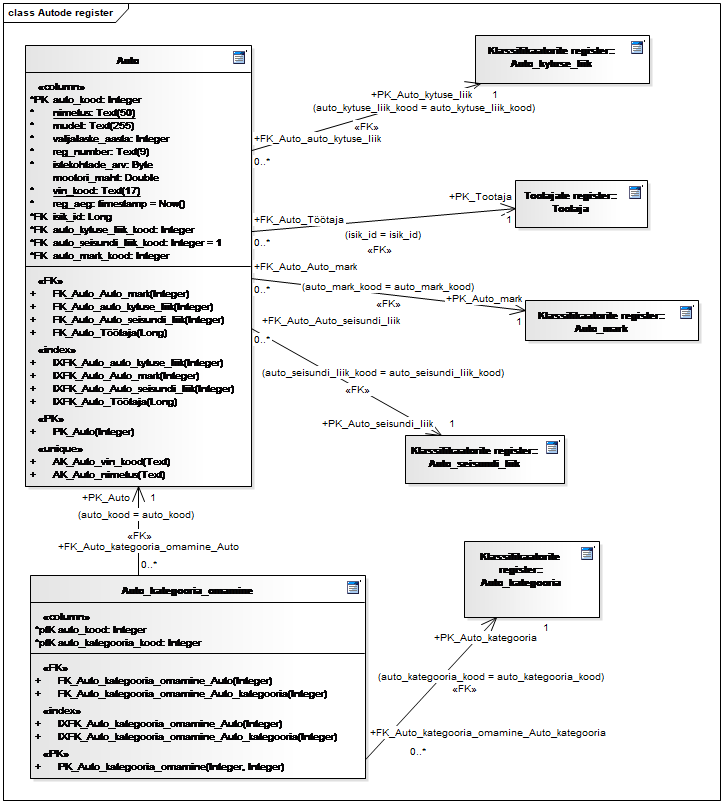
\includegraphics[scale=1]{joonis10}
	\caption{\textbf{Joonis 10. Autode registri füüsilise disaini andmebaasi diagramm}}
\end{figure}

\begin{figure}[H]
	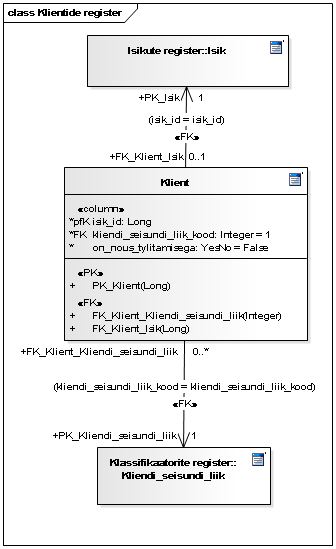
\includegraphics[scale=1]{joonis11}
	\caption{\textbf{Joonis 11. Klientide registri füüsilise disaini andmebaasi diagramm}}
\end{figure}
	
\begin{figure}[H]
	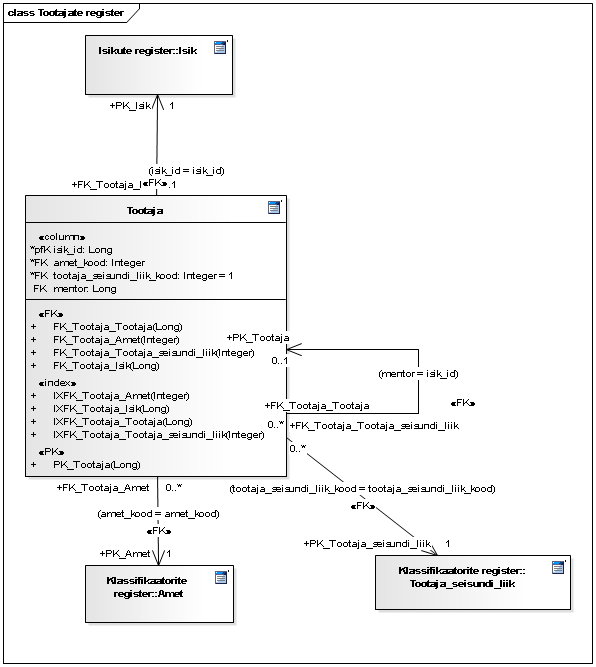
\includegraphics[scale=1]{joonis12}
	\caption{\textbf{Joonis 12. Töötajate registri füüsilise disaini andmebaasi diagramm.}}
\end{figure}

\begin{figure}[H]
	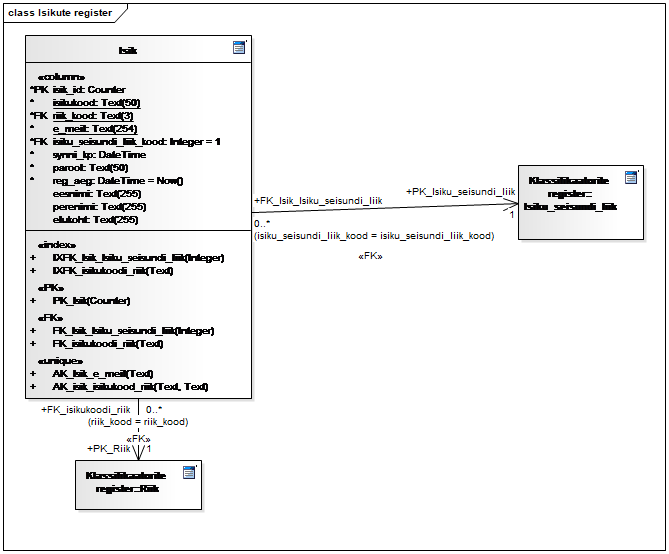
\includegraphics[scale=1]{joonis13}
	\caption{\textbf{Joonis 13. Isikute registri füüsilise disaini andmebaasi diagramm.}}
\end{figure}

\begin{figure}[H]
	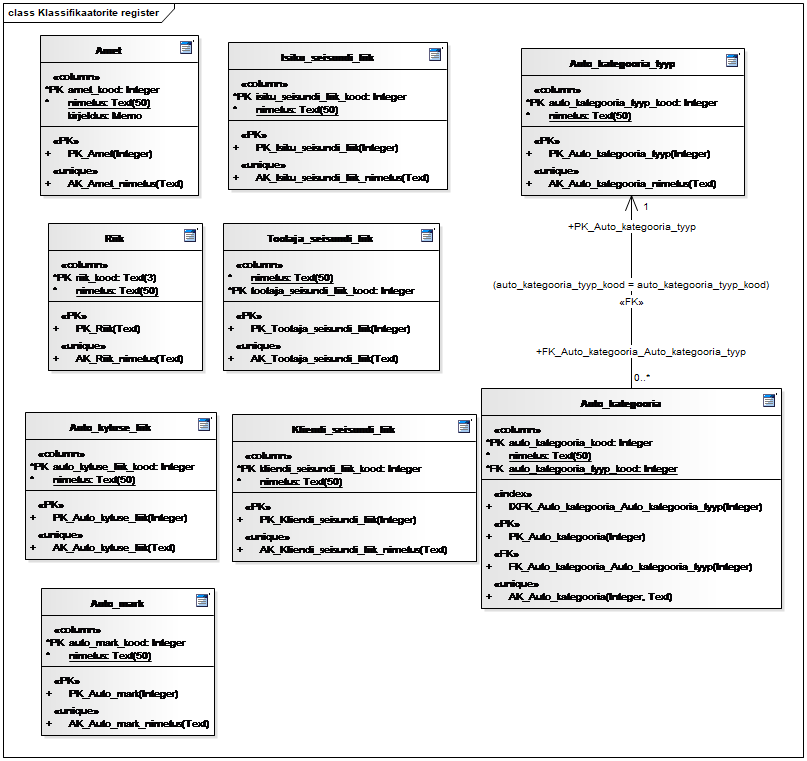
\includegraphics[scale=1]{joonis14}
	\caption{\textbf{Joonis 14. Klassifikaatorite registri füüsilise disaini andmebaasi diagramm.}}
\end{figure}